\section{Examples}
\label{sec:example}

%We now present a series progressing in complexity to demonstrate our approach. Our examples are from real Java Platform, Micro Edition (JME) formerly known as J2ME and Android API. Both JME and Android use Java as the language of implementation and targeted towards hand-held devices. However, our approach is independent of language of implementation and thus can be used for any similar source and target API.  

%First we parse the API documents of source and target API library and store it in intermediate representation for analysis. In particular, we extract class, interface and corresponding method descriptions from API documents. Second, we then create a term vector representation of each class description and method descriptions. Vector space model or term vector model is an algebraic model for representing text documents (and any objects, in general) as vectors of identifiers, such as, for example, index terms. In our case, each word is considered as a term barring the stop words such as (a, the, and ...). 

%Finally we use the term vector representation of a method description in a source API to query term vector representation of the the method description in target API. The results are ranked based on the Term Frequency-Inverse Document Frequency (TF-IDF) measure. TF-IDF is a numerical statistic which reflects how important a word is to a document in a collection or corpus. It is often used as a weighting factor in information retrieval and text mining.

%We then collect the top 10 results from target API methods for each source API method. Figure~\ref{fig:excpAPIJ2ME} and Figure~\ref{fig:excpAPIAndroid} shows example of trivially similar API methods. Our search results return the Android API method shown in Figure~\ref{fig:excpAPIAndroid} as a first match for the JME method shown in Figure~\ref{fig:excpAPIJ2ME}. Notice the slightly different description for the methods in JME and Android API. Although, correct this is very trivial mapping. We next present a more complex example.  

\begin{figure}[t]
\begin{CodeOut}
\begin{alltt}
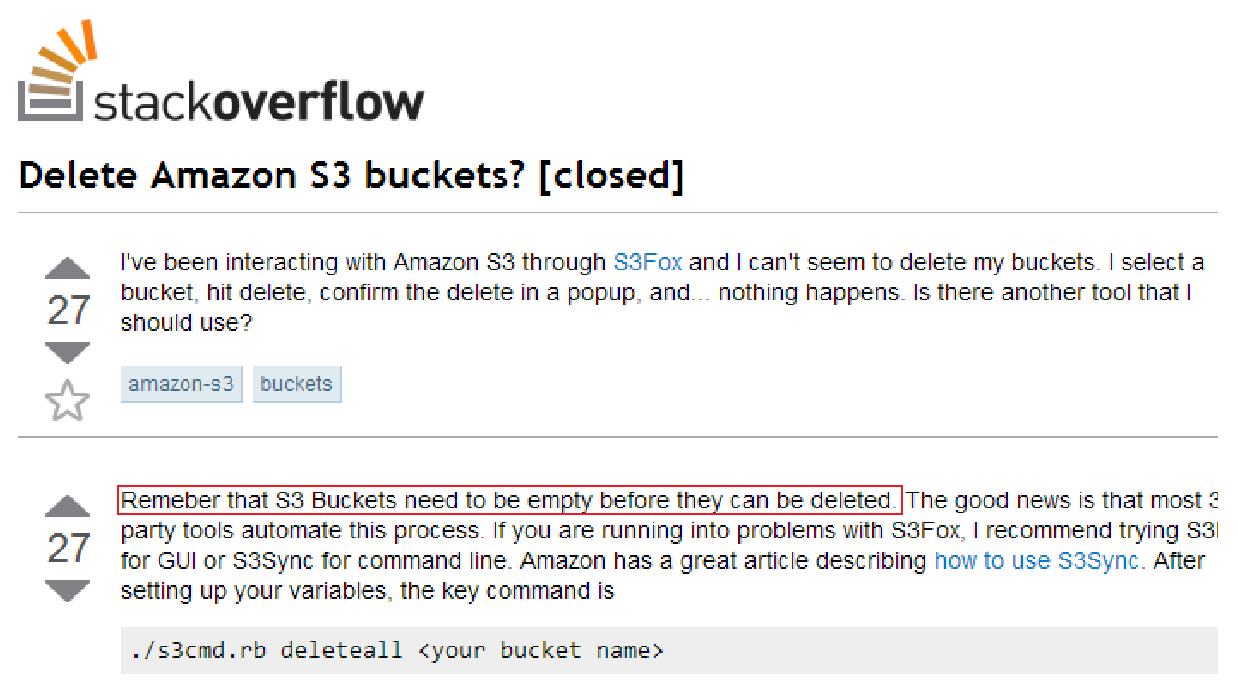
\includegraphics[scale=0.4]{Stackoverflow.eps}
\end{alltt}
\end{CodeOut}
\caption{\label{fig:Stackoverflow} The Query posted on Stackoverflow form regrading Amazon S3 REST API}
\end{figure}

\begin{figure}[t]
\begin{CodeOut}
\begin{alltt}
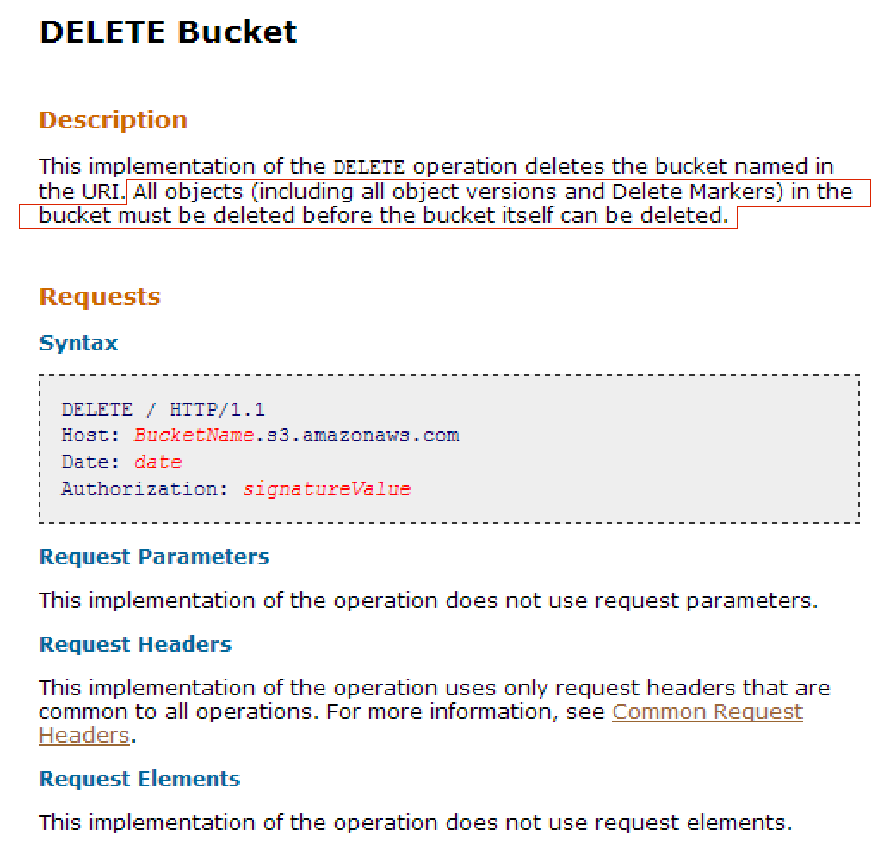
\includegraphics[scale=0.4]{AmzonS3DeleteBucketAPI.eps}
\end{alltt}
\end{CodeOut}
\caption{\label{fig:AmzonS3DeleteBucketAPI} The online API document for \CodeIn{DELETE Bucket} operation in Amazon S3 REST API}
\end{figure}


%Figure~\ref{fig:drawCharAPIJ2ME} and Figure~\ref{fig:drawTextAPIJ2ME} shows example of non-trivially similar API methods. Although, the textual description is similar using text analytics (TF-IDF similarity using term frequency vector), there is difference in type of arguments.

